\chapter{Java Memory Model}
A \textbf{memory model} for \textit{multithreaded} systems specifies how mem actions in a program will appear to execute to the programmer, i.e. {---}more specifically{---} which value each read of a memory location may return.\\
Every hardware and software interface of a system that admits multithreaded access to shared memory \textbf{requires} a memory model determining the transformations that the system can apply to a program.

{In the case of high-level programming languages such as Java the memory model determines\ns
\begin{enumerate}
   \item the transformations the compiler may apply to a program when \textbf{producing bytecode}
   \item the transformations a Virtual-Machine may apply to bytecode when \textbf{producing native code}
   \item The \textbf{optimizations} that hardware may perform on the native
\end{enumerate}}
Besides, the model also impacts the programmer,
since such transformations determine the possible outcomes of a program.\\
Without a well defined memory model for a programming language, it is impossible to known what the legal results are for a program in such language.
\note{When programming \textit{``correctly"} in Java, using \texttt{volatile} keywords and related constructs, we can {---}in some sense{---} ignore the memory model}

\framedt{Memory Hierarchy}
{In modern architectures memory is stratified ranging from mass memory (hard disks) to \texttt{CPU} registers, passing through different cache levels (\texttt{L1,L2,L3}),
obtaining a \textbf{memory hierarchy};
depending on \texttt{CPU} architectures, cache levels may be shared or not among cores.}

\section{Java Memory Model}
The JMM ---updated with Java 5--- first of all, provides standard guarantees for \textit{correctly synchronized} programs, i.e. sequential consistency of data-race-free programs.\\
For what concerns \textit{incorretly synchronized} programs instead, the behaviour is \textit{bounded} by a well-defined notion of \textbf{causality},
so the semantics are \textit{not} completely undefined as they were in the early (pre \texttt{Java 5} - $2004$) versions of the memory model.\\
The causality constraints are \textit{strong enough} to \textit{respect} the \textbf{safety} and \textbf{security} \textbf{properties} of java,
and \textit{weak enough} to \textit{allow} standard compiler and hardware \textbf{optimizations}.

\subsection{Runtime Data Areas}
\textbf{Local} {-}\textit{primitive} type{-} \textbf{variables} of methods are allocated on \ul{thread stacks},
and \textit{cannot} be accessed by other threads;
\textit{Objects} are instead allocated on the \ul{Heap}, and are the only ones which can be shared among threads.

\newpage
\begin{paracol}{2}

   \begin{figure}[htbp]
      \centering
      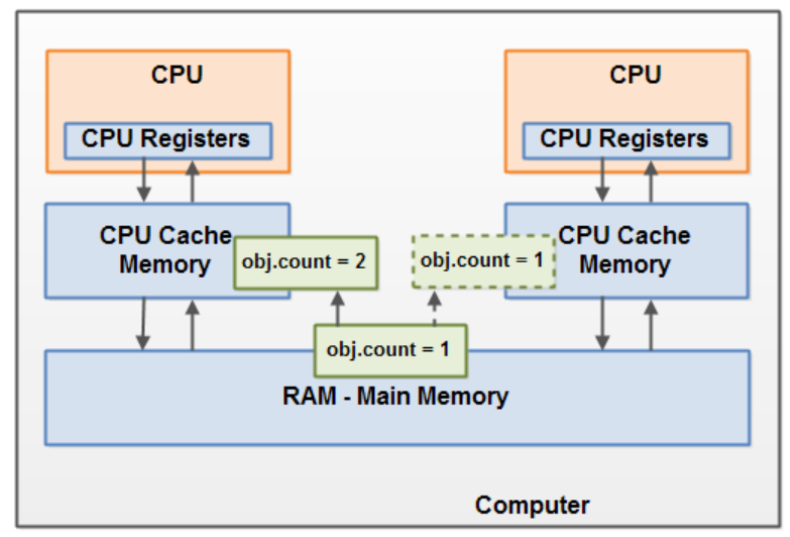
\includegraphics{images/jmm_visibility.png}
      \caption{Visibility issues across memory areas}
      \label{fig:jmm_visibility}
   \end{figure}

   
\end{paracol}
For what concerns the distribution of data in Java,
it may be spread orthogonally around the memory hierarchy, 
i.e. anything can go anywhere.\\
Access to shared variables, possibly in different memory areas,
leads to two key issues:
\begin{enumerate}
   \item \textbf{Visibility} of variable updates
   \item \textbf{Data Races}
\end{enumerate}
To overcome these issues Java provides the \lstinline|volatile| modifier, and \lstinline|synchronized methods/blocks|, which are explicitly taken into account by the JMM.


\section{\texttt{volatile} modifier}
\lstinline|volatile| is a modifier that can only be applied to fields of a class,
and intuitively it declares that a field can be modified by multiple threads\footnote{Clearly incompatible with \lstinline|final|}.
The JMM guarantees that the write of a volatile variable is visible when it is read.
An \textit{implementation} should guarantee that the new value is flushed from the cache to the RAM, if a read happens "after" a write.

\begin{center}
   What does it mean that \textit{``a read happens after a write''}?
\end{center}
This will be discussed later on in Sec \ref{sec:behaviour_actions}, however,
When threads do \textit{not} use any synchronization mechanism,
their behavior is described as the sequence of performed read/write \textbf{actions},
along with the results of the read operations;
such sequence has a \textbf{partial ordering} whose \textit{legitimacy} is checked by the JMM
which aims to \ul{ensure that a read results in the actual last value written in this partial ordering}.

\subsection{Data Races}
Notice that \lstinline|volatile| doesn't solve \textbf{Data Races}, which need synchronization mechanism;
the typical example is incrementing a shared counter, which actually consists of three operations, \texttt{read}, increment the value read, and \texttt{write} it;
such actions are \textbf{not} performed \textit{atomically}\footnote{So\dots which operations are atomic and which are not?},
thus a second thread may read the ``old'' before the first one writes the updated one, 
resulting in only one incrementation instead of two.

\subsection{Monitors}
Monitors are the default Java synchronization mechanisms.
Every object has a monitor exposing a lock which can be held only by one thread at a time.
methods and \dots with the \lstinline|synchronized| modifier are guarded by the lock.

\section{Describing thread behaviour}
\label{sec:behaviour_actions}
The JMM has no explicit global ordering of all actions by time consistent with each thread's perception of time, and has no global store.\\
Executions are instead described in terms of memory \textbf{actions},
\textbf{partial orders} on these actions, and a \textbf{visibility function} that assigns a write action to each read action.

\labelitemize{
   \textit{Actions}
}{
\begin{enumerate}
	\item \textred{Volatile read}
	\item \textred{Volatile write}
	\item \textred{Lock on monitor} $m \in \mathbb{M}$
	\item \textred{Unlock of monitor} $m \in \mathbb{M}$
	\item Normal read from $v \in \mathbb{L}$
	\item Normal write to $v \in \mathbb{L}$
	\item External action
   \item[] \note{Here \textred{``Synchronization''} actions are marked in \textred{red}.}
\end{enumerate}
}


An execution of a \textit{single-threaded} program fixes a total order $\leq_{po}$ on its \textit{actions}, called \textbf{program order};
while for a \textit{multi-threaded} the program order consists in the union the program order of its threads,
so it does not relate actions of different threads.\\
An execution of a \textit{multi-threaded} program is \textbf{sequentially consistent} if there is a total order of its actions consistent with the program order {---}and such that each read has the value of the last write{---}.\\
For \textit{datarace-free}\footnote{Also called \textit{\underline{corretly}} or \textit{\underline{well} synchronized programs}} mt-programs, the JMM guarantees that only \textbf{sequential consistent} executions are legal.

{JMM has been designed to guarantee three things:\ns
\begin{enumerate}
   \item \ul{Promise for programmers}\\
   Sequential consistency must be sacrificed to allow optimizations, 
   but it still holds for datarace-free program
   \item \ul{Promise for security}\\
   Values should not appear ``out of thin air'', allowing for information leakage
   \note{Even for non-datarace-free programs!}
   \item \ul{Promise for compilers}\\
   HW and SW optimizations should be applied without violating (both) the first two requirements
\end{enumerate}}

\subsection{Sequential Consistency is too strong}
\begin{paracol}{2}
   \begin{lstlisting}[caption={Thread 1}]
      int r1; 
      r1 = B;
      A = 1;
   \end{lstlisting}
\switchcolumn
   \begin{lstlisting}[caption={Thread 2}]
      int r2; 
      r2 = A;
      B = 1;
   \end{lstlisting}
\end{paracol}
Which values can \lstinline|r1| and \lstinline|r2| take?\\
Depends on who writes first, but in a \textit{sequentially consistent} execution, \lstinline|r1 == r2 == 1| is not possible.\\
However, it may occur in case of \textbf{instruction reordering}.
Conceptually, in the absence of synchronization, the compiler/JVM/CPU is
allowed to reorder the instructions (typically to improve performance) as
long as this reordering is irrelevant from the point of view of the single thread.\\
Indeed, if the order of the instructions of Thread 1 and/or Thread
2 is reversed, the result \lstinline|r1 == r2 == 1| becomes possible.


% Instr reordering may be performed as long as it guarantees sequential consistency in the \textit{single thread}

\subsection{Out-of-thin-air}
\begin{paracol}{2}
   \begin{lstlisting}[caption={Thread 1}]
      r1 = x;
      y = r1;
   \end{lstlisting}
\switchcolumn
   \begin{lstlisting}[caption={Thread 2}]
      r2 = y;
      x = r2;
   \end{lstlisting}
\end{paracol}
\lstinline|x = y = 0| initially;
can we obtain \lstinline|r1 == r2 == 42| at the end?\\
\textit{"Well \textbf{no}, but actually \textbf{yes}\dots"}\\
In some situations the Runtime environment may \textit{guess} that, 
at some point, \lstinline|x| evaluates to \lstinline|42|:
we say that \lstinline|42| comes \textit{"out-of-thin-air"}.
Then it checks by looking at the two thread instructions if it may happen that \lstinline|r1 == r2 == 42|:
\begin{center}
   "Yes! So x actually really evaluates to 42! I guessed right! \smiley"
\end{center}
This was an accepted guess before the JMM introduced with Java 5 (2004),
but currently such claims at runtime are forbidden.

\subsection{Synchronization order}
{Each execution of a program is associated with a \textbf{synchronization order} $\leq_{so}$ which is \ul{a total order over all \textit{synchronization} actions} satisfying:\ns
\begin{enumerate}
   \item Consistency with program order
   \item Read to a volatile variable $v$ returns the value of the write to $v$ that is ordered last before the read by the synchronization order.
\end{enumerate}}

{$a \leq_{sw} b$ is read ``action $a$ synchronizes with action $b$''. This holds if $a \leq_{so} b$ \ul{and}:\ns
\begin{itemize}
   \item $a$ unlocks a monitor and $b$ locks it
   \item $a$ writes to a \lstinline|volatile| variable and $b$ reads it
\end{itemize}
}

Relation \textit{\textbf{happens-before}} $\leq_{hb}$ is the ---(smallest relation)--- \textbf{transitive closure} of the \textit{program order} $\leq_{po}$ and the \textit{synchronizes-with} $\leq_{sw} relation.$
$A \leq_{hb} B$ means that $A$ is guaranteed to be \textit{visible} to $B$ in the execution.\\
If $A \leq_{po} B$ (same thread), or $A \leq_{sw} B$ (synchronization), then $A \leq_{hb} B$.\\
It is the transitive closure in the sense that if $A \leq_{hb} B$ and $B \leq_{hb} C$, then $A \leq_{hb} C$.

\subsection{Formally Defining Data Races}
\begin{definition}
   [Data Race]
   Two accesses $x$ and $y$ form a data race in an execution of a program if they are from different threads, they conflict, and they \ul{are not ordered by happens-before} in a sequential consistent execution.
\end{definition}

A program is said to be \textbf{correctly synchronized} ---or datarace-free--- if and only if all sequentially consistent executions of the program are free of data races.

The first requirement for the JMM is to ensure sequential consistency for correctly synchronized or datarace free programs\\
\ul{Programmers should not worry about code transformations for datarace-free programs}.

% \labelitemize{\textit{Executions - Formal Definition}}
% {
%    $E = (P,A,\leq_{po},\leq_{so},W,V,\leq_{sw},\leq_{hb})$
%    \begin{enumerate}
%    \item 
%    TODO
% \end{enumerate}}
\begin{figure}[htbp]
   \centering
   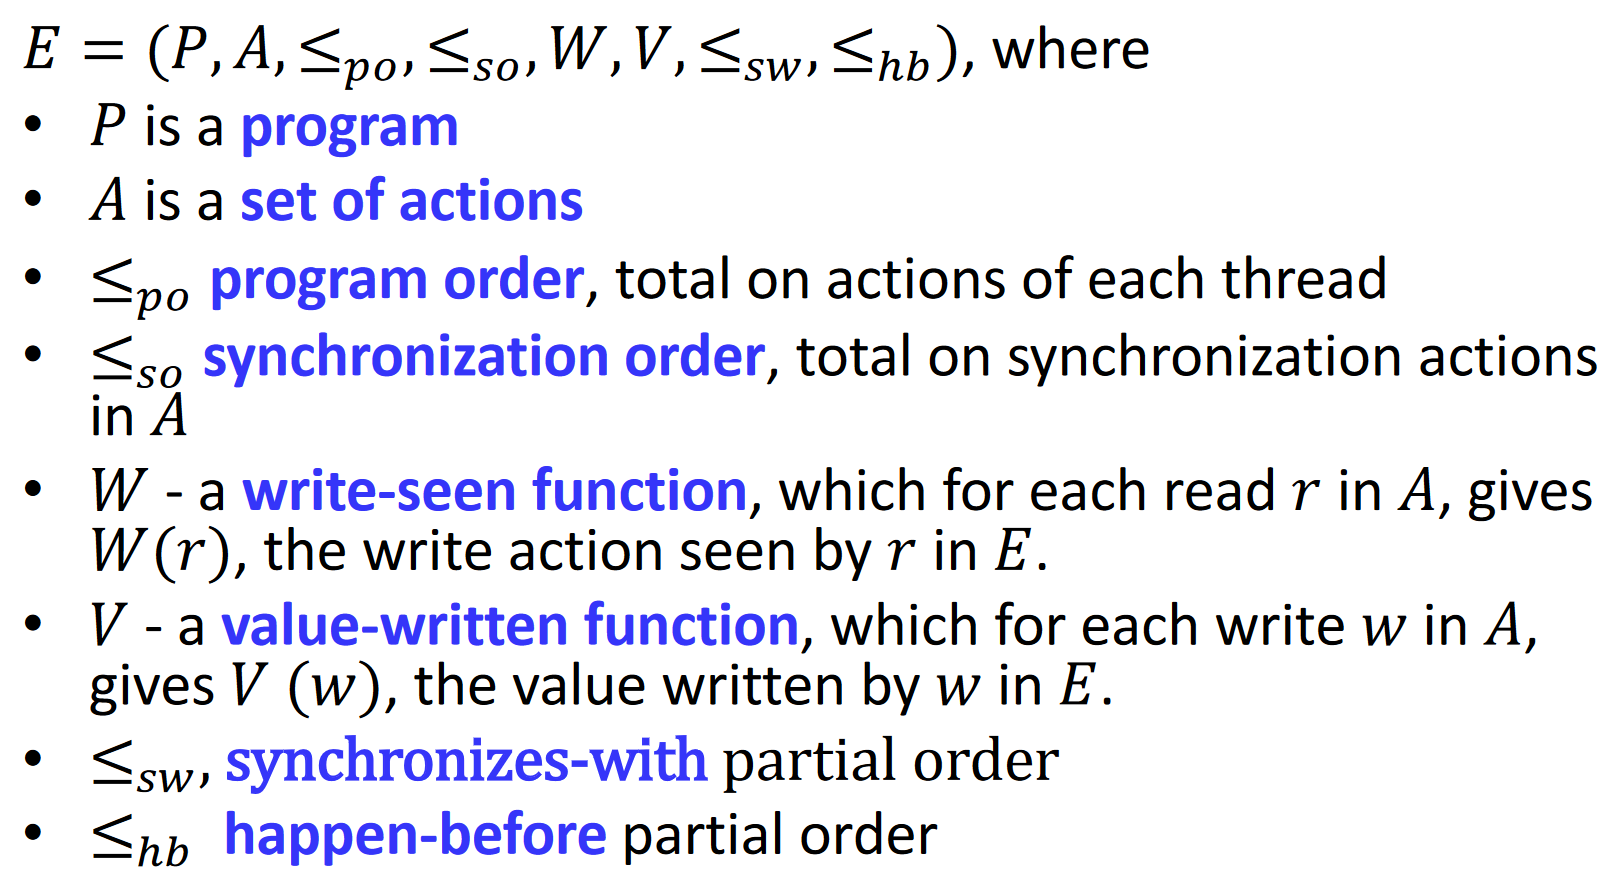
\includegraphics{images/jmm_dataraces.png}
   \caption{Dataraces Formally}
   \label{fig:jmm_dataraces}
\end{figure}



$E = (P,A,\leq_{po},\leq_{so},W,V,\leq_{sw},\leq_{hb})$ is a \textbf{well-formed execution} if:
\begin{enumerate}
   \item Each read of a var $x$ sees a write to $x$, and all reads and writes of volatile variables are volatile actions
   \item Synchronization order is consistent with program order and mutual exclusion
   \note{If thread $T_1$ performs synchronization actions $A$ and $B$ in that order, then $A$ must appear before $B$ in the synchronization order}
   \item The execution obeys intra-thread consistency
   \item The execution obeys intra-thread and happens-before consistency (each read of $v$ sees the last preceding write to $v$)
\end{enumerate}

Now, which \textit{well-formed executions} are \textbf{legal}?
\textbf{Legal executions} are built iteratively:
in each iterations, the JMM commits a set of memory actions;
actions can be committed if they occur in some well-behaved execution that also contains the actions
committed in previous iterations.
The JMM must ensure that appropriate executions are prohibited.

A well-formed $E = (P,A,\leq_{po},\leq_{so},W,V,\leq_{sw},\leq_{hb})$ is validated by \textit{commiting} actions in A;
if all actions of A are committed, then E is legal.
``Committing actions'' means progressively building up a valid execution by considering subsets of actions, starting with none and ending with the entire set AA

There must exists a sequence of subsets of a
\[
  C_0 \subset C_1 \subset \dots \subset C_n = A 
\]
Where each $C_i$ is a progressively larger subset of committed actions in $A$. $C_0 = \emptyset$ and $C_n = A$ (all actions are committed in the final step).

For each $C_i$ there is one $\{E_i\}_{i\leq n}$ of well-formed executions such that each $E_i$ ``witnesses'' the actions in $C_i$, meaning that $E_i$ show how those actions can be legally executed under the JMM.
\ul{Any reads, writes, or synchronization in $C_i$ must be consistent with the program order, synchronization order, and happens-before relationships in $E_i$.}

If you can construct such a sequence of subsets $C_i$ and corresponding well-formed executions $E_i$, then the entire execution EE is legal under the JMM.

\note{
   % // TODO
I did not understand this witnessing part honestly\dots}

\begin{figure}[htbp]
   \centering
   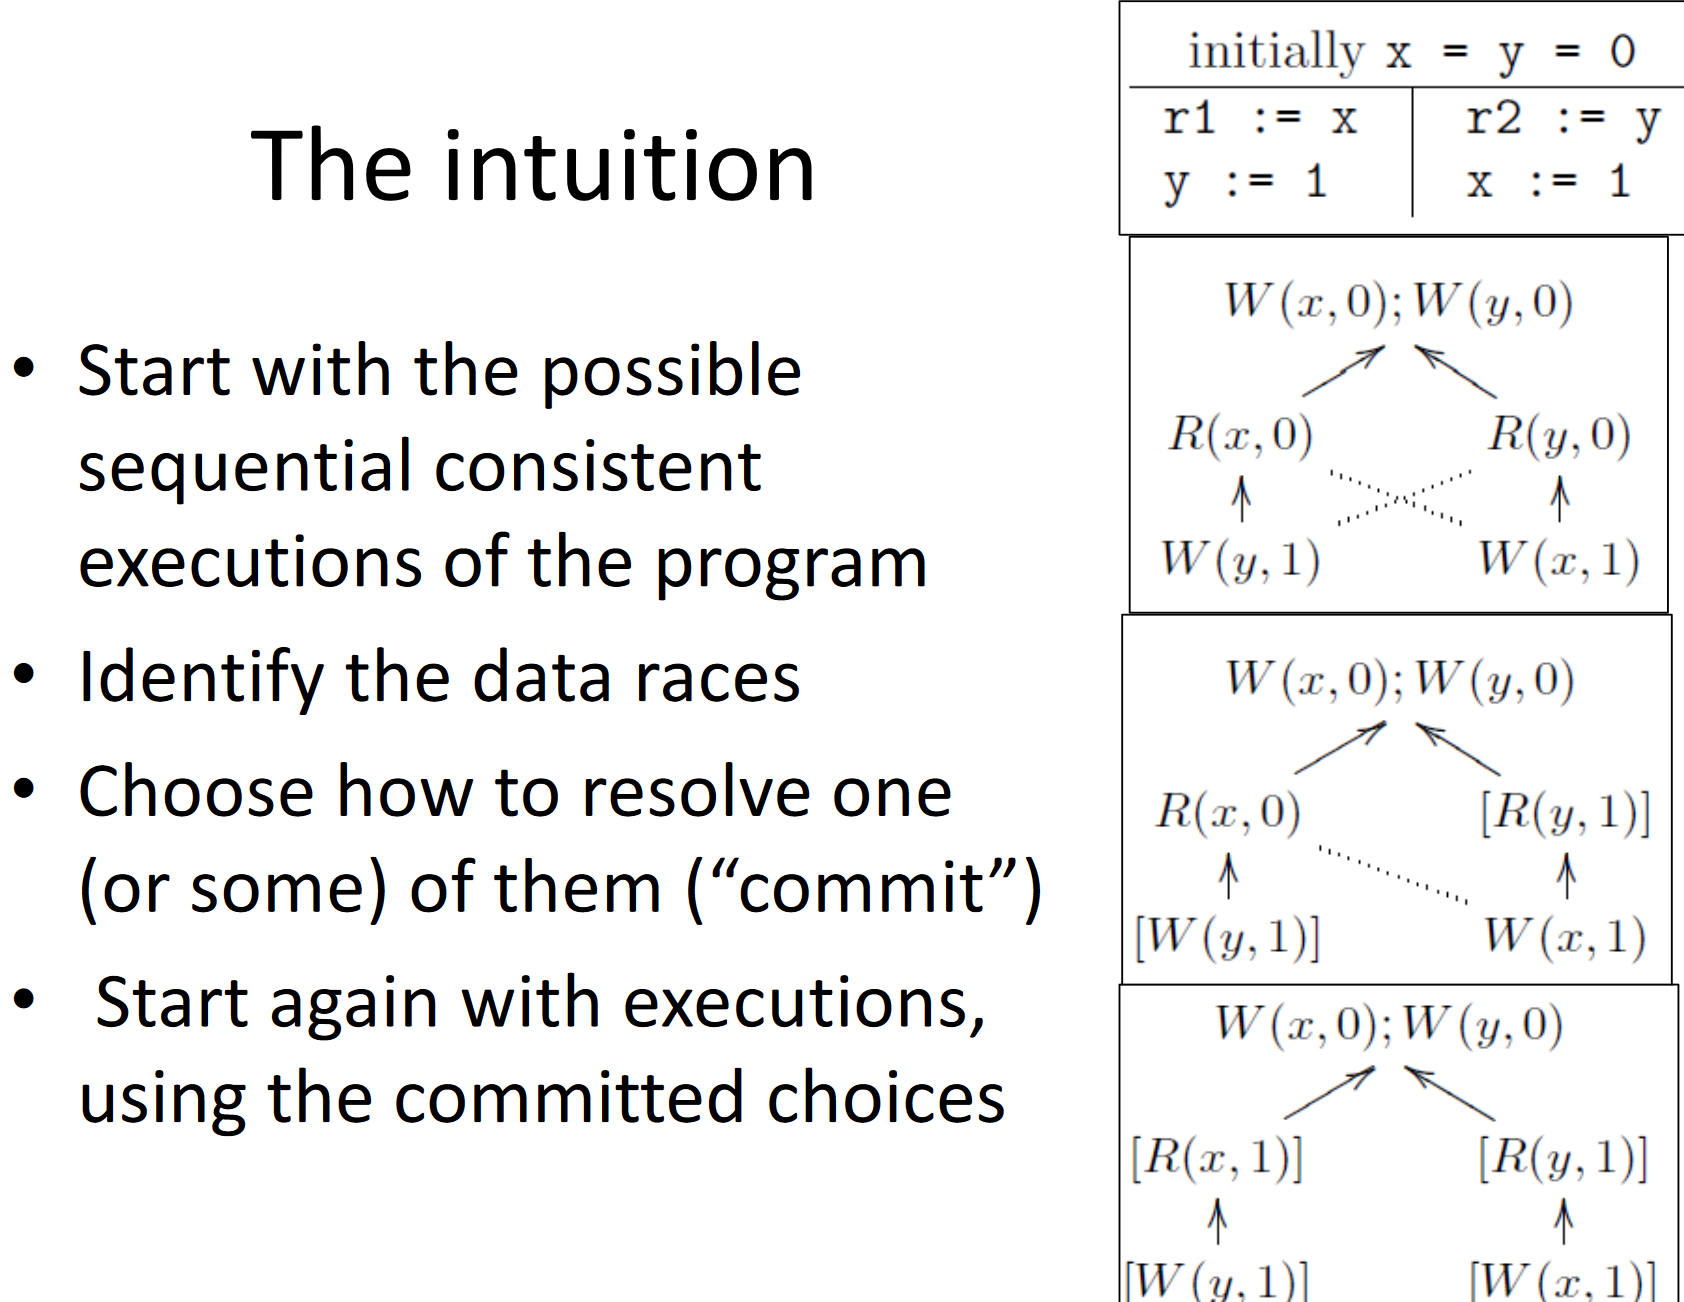
\includegraphics{images/legal_executions.png}
   \caption{Legal Executions}
   \label{fig:legal_executions}
\end{figure}

\section{Rules for Java Programmers}
Even disregarding the technicalities of the model, its
impact can be translated to a set of useful rules for
{Java programmers, which may be of three types:\ns
\begin{itemize}
	\item \textbf{Atomicity} - Which operations are naturally atomic?
	\item \textbf{Visibility} - When does a memory write become
visible to other threads?
	\item \textbf{Reordering} - In what order can the operations be
rearranged?
\end{itemize}}

\subsection{Atomicity}
An operation is \textbf{atomic} if, from the point of view of any other thread, its effects are seen in full, or not at all (but never ``half'').But then\dots\\
Which operations are naturally atomic, even in the absence of mutual
exclusion mechanisms?\\
{JLS and JMM guarantee that:\ns
\begin{itemize}
   \item Reads and writes of \texttt{reference} variables are atomic
   \item Reads and writes of \texttt{primitive} variables are atomic, \textit{except} for \texttt{long} and \texttt{double} variables
   \note{Modification of a long variable can occur in two distinct operations which may be interrupted by the scheduler, separately modifying the 32 most significant bits and the 32 least significant bits.}
   \coolquote{Implementations of the Java Virtual Machine are encouraged to avoid splitting 64-bit values where possible. Programmers are encouraged to declare shared 64-bit values as volatile or synchronize their programs correctly to avoid possible complications. }{JSL 17}
   \item Reads and writes of \texttt{volatile} variables are atomic
\end{itemize}}

\begin{lstlisting}
   int x, y;
   long n;
   volatile long m;
   Object a, b;
   volatile Object c, d;
   
   1. x = 8;                  // Atomic
   2. x = y;                  // Atomic
   3. n = 0x1122334455667788; // Not Atomic
   4. m = 0x1122334455667788; // Atomic
   5. m++;                    // Not Atomic
   6. a = null;               // Atomic
   7. a = b;                  // Atomic
   8. c = d;                  // Atomic
\end{lstlisting}

Note that volatile modifier makes only a single write to
the variable in question atomic:
even if \lstinline|a| and \lstinline|b| are both \lstinline|volatile|, \lstinline|a = b| is \textbf{not} atomic.

\subsection{Visibility}
In absence of synchronization, the operations (writes to memory)
performed by a thread can remain hidden from other threads \textbf{indefinitely}.
In particular, some operations may remain hidden, and others may be
visible.

{Visibility is guaranteed by the following operations:\ns
\begin{itemize}
   \item Acquiring a \textbf{monitor} (i.e., entering a \lstinline|synchronized| method or block) makes visible the operations performed by the last thread that owned that monitor, up until the moment it released it
   \item Reading the value of a \lstinline|volatile| variable makes visible the operations carried out by the last thread that modified that variable, up to the moment in which it modified it
   \item Invoking \lstinline|t.start()| makes visible to the new thread \lstinline|t| all the operations carried out by the calling thread, up to the invocation of start
   \item Returning from a \lstinline|t.join()| invocation makes visible all the operations carried out by thread t until its termination 
\end{itemize}
}

\subsection{Reordering}
As said, the compiler, the JVM and the CPU can reorder any
sequence of instructions as long as the result does not change for
the single thread.
Clearly, \lstinline|synchronized| and \lstinline|volatile| constructs reduce the possibility of reordering, but we can dig deeper.

Consider two subsequent instructions \lstinline|x1| and \lstinline|x2| having no dependencies between them from the point of view of a single thread.
In which cases may they be ---reversed--- reordered?

\begin{paracol}{2}
   
   \begin{figure}[htbp]
      \centering
      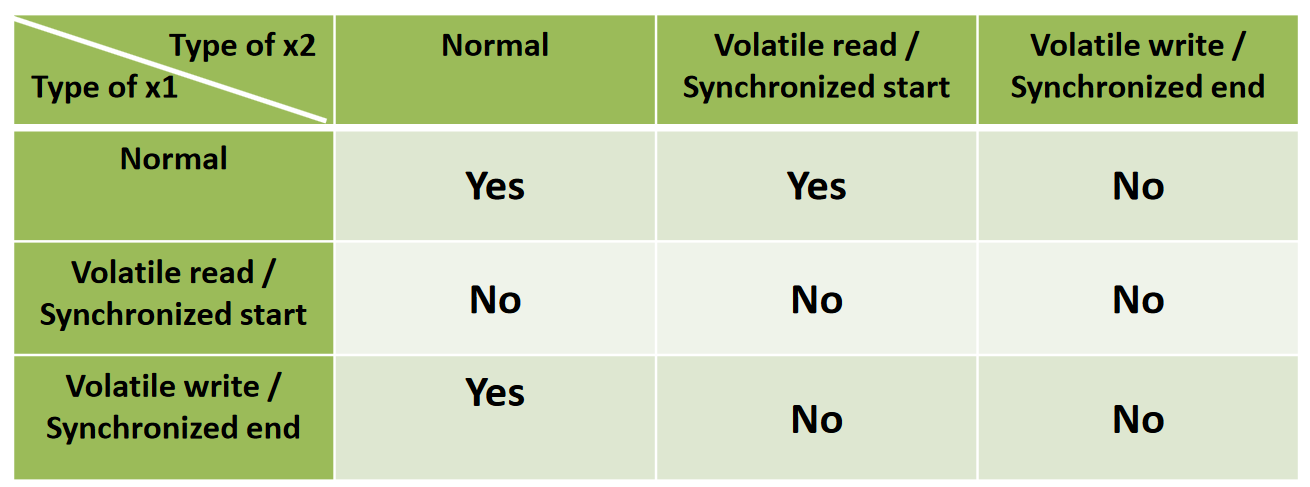
\includegraphics{images/jmm_reordering.png}
      \caption{Reodering \lstinline|x1,x2|cases}
      \label{fig:jmm_reordering}
   \end{figure}

   \switchcolumn
\begin{itemize}
	\item Normal instructions can always be interchanged
	\item Normal instructions can be brought into a synchronized block
	\item The normal instructions that precede the reading of a volatile can be moved after the reading
	\item The normal instructions that follow the writing of a volatile can be moved before the writing
\end{itemize}
\end{paracol}